\documentclass[border=15pt, tikz]{standalone}
\usepackage[T1]{fontenc}
\usepackage[utf8]{inputenc}
\usepackage{tikz}
\usetikzlibrary{positioning, arrows.meta, decorations.pathreplacing, calc, fit}
\definecolor{clrattention}{HTML}{45B7D1}
\definecolor{clrattention_alt}{HTML}{96E6F0}
\definecolor{clrffn}{HTML}{F97068}
\definecolor{clrnorm}{HTML}{FFD93D}
\definecolor{clrembed}{HTML}{6BCB77}
\definecolor{clrresidual}{HTML}{4D96FF}
\definecolor{clroutput}{HTML}{C084FC}
\definecolor{clrspectral}{HTML}{22D3EE}
\definecolor{clrphysics}{HTML}{FB923C}
\definecolor{clrborder}{HTML}{334155}
\definecolor{clrtext}{HTML}{1E293B}
\definecolor{clrgroup_frame}{HTML}{94A3B8}
\definecolor{clrgroup_fill}{HTML}{F1F5F9}
\begin{document}
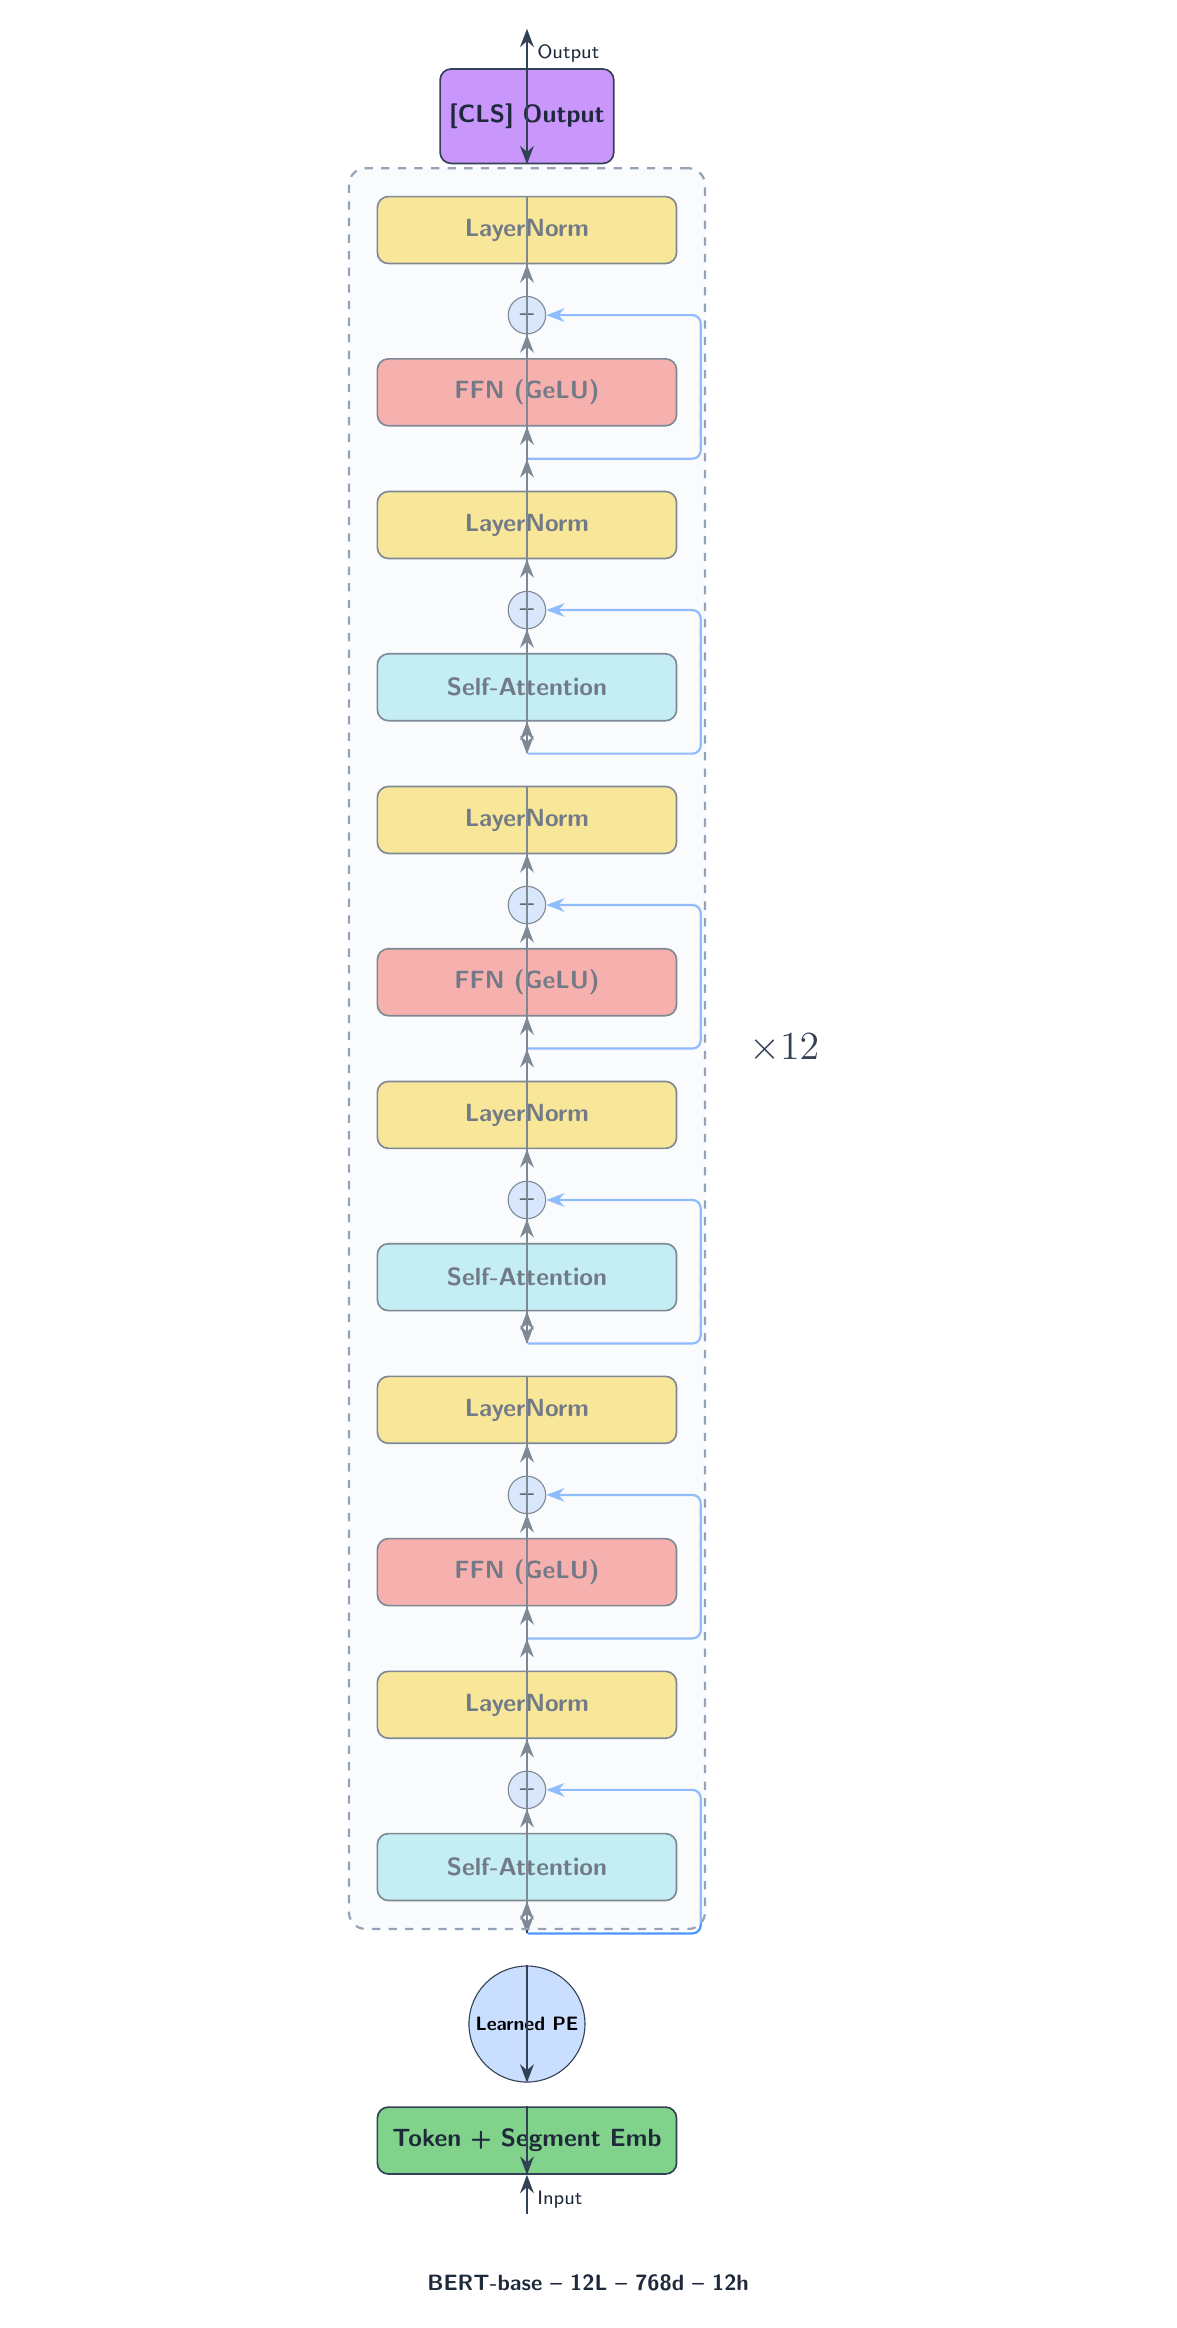
\begin{tikzpicture}[
    >=Stealth,
    every node/.style={font=\sffamily},
    block/.style={draw=clrborder, rounded corners=4pt, minimum width=3.8cm,
                  minimum height=0.85cm, font=\sffamily\small\bfseries,
                  text=clrtext, line width=0.6pt},
    arrow/.style={->, thick, color=clrborder, line width=0.8pt},
    skiparrow/.style={->, thick, color=clrresidual, line width=0.8pt, rounded corners=3pt},
    label/.style={font=\sffamily\scriptsize, text=clrtext},
    subtitle/.style={font=\sffamily\footnotesize, text=clrtext},
]
\node[block, fill=clrembed!85, minimum width=3.8cm, minimum height=0.85cm, text=clrtext] (n_1) at (0,0) {Token + Segment Emb};
\node[circle, draw=clrborder, fill=clrresidual!30, inner sep=2pt, font=\sffamily\scriptsize\bfseries, above=0.3cm of n_1] (n_2) {Learned PE};
\node[inner sep=0, minimum size=0, above=0.4cm of n_2] (res_entry_3) {};
\node[block, fill=clrattention_alt!85, minimum width=3.8cm, minimum height=0.85cm, text=clrtext, above=0.4cm of res_entry_3] (n_4) {Self-Attention};
\node[circle, draw=clrborder, fill=clrresidual!30, inner sep=2pt, font=\sffamily\scriptsize\bfseries, above=0.3cm of n_4] (add_5) {+};
\node[block, fill=clrnorm!85, minimum width=3.8cm, minimum height=0.85cm, text=clrtext, above=0.4cm of add_5] (n_6) {LayerNorm};
\node[inner sep=0, minimum size=0, above=0.4cm of n_6] (res_entry_7) {};
\node[block, fill=clrffn!85, minimum width=3.8cm, minimum height=0.85cm, text=clrtext, above=0.4cm of res_entry_7] (n_8) {FFN (GeLU)};
\node[circle, draw=clrborder, fill=clrresidual!30, inner sep=2pt, font=\sffamily\scriptsize\bfseries, above=0.3cm of n_8] (add_9) {+};
\node[block, fill=clrnorm!85, minimum width=3.8cm, minimum height=0.85cm, text=clrtext, above=0.4cm of add_9] (n_10) {LayerNorm};
\node[inner sep=0, minimum size=0, above=0.4cm of n_10] (res_entry_11) {};
\node[block, fill=clrattention_alt!85, minimum width=3.8cm, minimum height=0.85cm, text=clrtext, above=0.4cm of res_entry_11] (n_12) {Self-Attention};
\node[circle, draw=clrborder, fill=clrresidual!30, inner sep=2pt, font=\sffamily\scriptsize\bfseries, above=0.3cm of n_12] (add_13) {+};
\node[block, fill=clrnorm!85, minimum width=3.8cm, minimum height=0.85cm, text=clrtext, above=0.4cm of add_13] (n_14) {LayerNorm};
\node[inner sep=0, minimum size=0, above=0.4cm of n_14] (res_entry_15) {};
\node[block, fill=clrffn!85, minimum width=3.8cm, minimum height=0.85cm, text=clrtext, above=0.4cm of res_entry_15] (n_16) {FFN (GeLU)};
\node[circle, draw=clrborder, fill=clrresidual!30, inner sep=2pt, font=\sffamily\scriptsize\bfseries, above=0.3cm of n_16] (add_17) {+};
\node[block, fill=clrnorm!85, minimum width=3.8cm, minimum height=0.85cm, text=clrtext, above=0.4cm of add_17] (n_18) {LayerNorm};
\node[inner sep=0, minimum size=0, above=0.4cm of n_18] (res_entry_19) {};
\node[block, fill=clrattention_alt!85, minimum width=3.8cm, minimum height=0.85cm, text=clrtext, above=0.4cm of res_entry_19] (n_20) {Self-Attention};
\node[circle, draw=clrborder, fill=clrresidual!30, inner sep=2pt, font=\sffamily\scriptsize\bfseries, above=0.3cm of n_20] (add_21) {+};
\node[block, fill=clrnorm!85, minimum width=3.8cm, minimum height=0.85cm, text=clrtext, above=0.4cm of add_21] (n_22) {LayerNorm};
\node[inner sep=0, minimum size=0, above=0.4cm of n_22] (res_entry_23) {};
\node[block, fill=clrffn!85, minimum width=3.8cm, minimum height=0.85cm, text=clrtext, above=0.4cm of res_entry_23] (n_24) {FFN (GeLU)};
\node[circle, draw=clrborder, fill=clrresidual!30, inner sep=2pt, font=\sffamily\scriptsize\bfseries, above=0.3cm of n_24] (add_25) {+};
\node[block, fill=clrnorm!85, minimum width=3.8cm, minimum height=0.85cm, text=clrtext, above=0.4cm of add_25] (n_26) {LayerNorm};
\node[block, fill=clroutput!85, minimum width=2.0cm, minimum height=1.2cm, text=clrtext, above=0.4cm of n_26] (n_27) {[CLS] Output};
\draw[arrow] (n_1.north) -- (n_1.south);
\draw[arrow] (n_2.north) -- (n_2.south);
\draw[arrow] (res_entry_3.north) -- (n_4.south);
\draw[arrow] (n_4.north) -- (add_5.south);
\draw[skiparrow] (res_entry_3.east) -- ++(2.2,0) |- (add_5.east);
\draw[arrow] (add_5.north) -- (n_6.south);
\draw[arrow] (res_entry_7.north) -- (n_8.south);
\draw[arrow] (n_8.north) -- (add_9.south);
\draw[skiparrow] (res_entry_7.east) -- ++(2.2,0) |- (add_9.east);
\draw[arrow] (n_6.north) -- (res_entry_7.south);
\draw[arrow] (add_9.north) -- (n_10.south);
\draw[arrow] (n_10.north) -- (res_entry_3.south);
\draw[arrow] (res_entry_11.north) -- (n_12.south);
\draw[arrow] (n_12.north) -- (add_13.south);
\draw[skiparrow] (res_entry_11.east) -- ++(2.2,0) |- (add_13.east);
\draw[arrow] (add_13.north) -- (n_14.south);
\draw[arrow] (res_entry_15.north) -- (n_16.south);
\draw[arrow] (n_16.north) -- (add_17.south);
\draw[skiparrow] (res_entry_15.east) -- ++(2.2,0) |- (add_17.east);
\draw[arrow] (n_14.north) -- (res_entry_15.south);
\draw[arrow] (add_17.north) -- (n_18.south);
\draw[arrow] (n_18.north) -- (res_entry_11.south);
\draw[arrow] (res_entry_19.north) -- (n_20.south);
\draw[arrow] (n_20.north) -- (add_21.south);
\draw[skiparrow] (res_entry_19.east) -- ++(2.2,0) |- (add_21.east);
\draw[arrow] (add_21.north) -- (n_22.south);
\draw[arrow] (res_entry_23.north) -- (n_24.south);
\draw[arrow] (n_24.north) -- (add_25.south);
\draw[skiparrow] (res_entry_23.east) -- ++(2.2,0) |- (add_25.east);
\draw[arrow] (n_22.north) -- (res_entry_23.south);
\draw[arrow] (add_25.north) -- (n_26.south);
\draw[arrow] (n_26.north) -- (res_entry_19.south);
\draw[arrow] (n_27.north) -- (n_27.south);
\draw[arrow] (n_1.south) ++ (0,-0.5) -- node[right, yshift=-2pt, font=\sffamily\scriptsize, text=clrtext] {Input} (n_1.south);
\draw[arrow] (n_27.north) -- node[right, yshift=-2pt, font=\sffamily\scriptsize, text=clrtext] {Output} ++ (0,0.5);
\node[draw=clrgroup_frame, rounded corners=6pt, dashed, line width=0.8pt, fill=clrgroup_fill, fill opacity=0.4, inner sep=0.35cm, fit=(n_4) (n_6) (n_8) (n_10) (n_12) (n_14) (n_16) (n_18) (n_20) (n_22) (n_24) (n_26)] (g_0) {};
\node[right=12pt of g_0.east, anchor=west, font=\sffamily\Large\bfseries, text=clrborder] (g_0_badge) {$\times12$};
\node[below=0.6cm of current bounding box.south, subtitle, text width=14cm, align=center] {\textbf{BERT-base -- 12L -- 768d -- 12h}};
\end{tikzpicture}
\end{document}
